% Created 2020-02-12 Wed 14:42
% Intended LaTeX compiler: pdflatex
\documentclass[11pt]{article}
\usepackage[utf8]{inputenc}
\usepackage[a4paper]{geometry}
\usepackage{graphicx}
\usepackage{amsmath}
\usepackage{amssymb}

\usepackage{tikz}

\usepackage{hyperref}
\usepackage{cleveref}
\date{\today}
\title{Enclave-NN}

% TODO: Fix terminology (provider, customer, model, etc.)}

\newcommand{\mail}{E-mail}
\newcommand{\tf}{TensorFlow}

\begin{document}

\maketitle
\tableofcontents

\begin{abstract}
In order to perform inference with a given machine learning model, the weights and architecture must be known.
Allowing a third party to query a model, while keeping it secret, requires providing the model as an online oracle to them.
While this allows keeping the model parameters private and thus continuing to monetize the model queries, it requires providing the infrastructure and computational power required to perform the inferences.

Our goal is to leverage the data confidentiality that Trusted Execution Environments (TEEs) promise to turn these online oracles into offline oracles, freeing the model creator from having to provide the infrastructure required for inference.
While the model creator benefits from the model parameters staying private, the model user can now also keep their inference data private, as they no longer have to provide them to the model creator for their inference.
Thus all involved parties gain privacy from such a model.

We provide a proof of concept implementation for certain Tensorflow operations, and provide a mechanism to cut the last \($n$\) layers and run them inside an Intel SGX enclave.
We then evaluated the performance impact of different cuts for four different neural net models.
This gives us an approximation for the impact caused by moving parts of the model to the CPU, and the additional impact introduced by the overhead of TEE execution.
\end{abstract}

\section{Introduction}
\label{sec:introduction}

Training a machine learning model requires large amounts of data, domain knowledge, and significant computation power.
Organizations wishing to use the predictive powers of these models often lack the knowledge and hardware required to train these models, and outsource parts of the task using Machine Learning as a Service (MLaaS) providers, who provide automated tools to generate ML models for certain types of tasks.

MLaaS providers usually monetize their models per query or per time frame.
Both strategies require them to keep the model parameters - and to some extent the architecture - secret.
A common strategy is to offer access to the finished model only as an online oracle which customers can query with their data, and which responds with the inference result.
Providing such an oracle requires the provider to continually reserve the needed computational power required for inference on the customer's model.
It also requires the customer to keep sending data to the provider at inference time, which can be undesirable and potentially illegal depending on the domain.
As such, the online oracle model required for continuous monetization is undesirable for both provider and customer.

Our approach transforms the online oracle into an offline oracle by leveraging the data confidentiality promised by trusted execution environments (TEEs).
We provide a (naive) implementation of different Tensorflow operations in C, as well as a tool to automatically generate the calls to these operations from an existing \tf{} model.
Our tool also extracts the weights from the model and makes them usable and protecting them inside the enclave.
We also provide an enclave wrapper which integrates seamlessly into \tf{}, making our enclave models drop-in replacements for regular \tf{} models.

While this approach still requires customers to share their training data with MLaaS providers, it allows us to leverage the higher performance of GPUs and optimized implementations of \tf{} operators during training.
Training a full model inside the enclave in order to provide data confidentiality during training time has been done \cite{ohrimenko_oblivious_2016}, but was not the goal for our research.
As evidenced by our results the performance impact of running a model inside the enclave can be quite large, especially for large convolutional neural nets (CNNs) as are commonly used in current image recognition tasks.
While these performance impacts could be acceptable during inference, depending on the application scenario, they seem to us be prohibitive during training, which caused us to use regular \tf{} on the GPU for training.

\section{Related Work}
\label{sec:related}

We have different areas of related work that are relevant to this project.
The most directly relevant area is model stealing attacks and adversarial robustness.
In model stealing an attacker tries to build a replicant model that rivals the prediction accuracy of the stolen model, with hopefully lower cost than using the original model.
Tramer et al.~\cite{tramer_stealing_2016} use a model-dependent dataset augmentation algorithm to find a reasonably low number of queries required for extracting the model.
The number they arrive at for NNs is \texttt{100*k}, where \texttt{k} is the number of parameters, making it infeasible for modern models which have millions of trainable parameters.

Another relevant area of research is adversarial attacks.
Papernot et al.~\cite{papernot_practical_2017} have presented a so-called black-box transfer attack, in which an attacker builds a local replicant model and builds adversarial examples on the gradients of that model.
This requires far less queries than are required for model stealing, but the replicant model does not have to be accurace.
Its only requirement is that its gradients are sufficiently aligned with the target model to build functional adversarial examples.

Our implementation affects data privacy, as it allows users to keep the data they wish to predict on private.
It also allows for the creation of offline black box oracles, which are used e.g. in set membership attacks by Shokri et al.~\cite{shokri_membership_2017}.
As it currently stands, we do not return confidence values, only the resulting label.
This makes the attack presented by Shokri et al. not better than chance, as evidenced by their own results.

In the context of data privacy Ohrimenko et al.~\cite{ohrimenko_oblivious_2016} have also previously combined machine learning with trusted enclaves.
The difference between their approach and ours is that they trained the model inside the enclave, which allows parties to also keep their training data private.
Their focus is on ensuring that no inference on the training data can be made using timing side channels, and they disregard performance.
Our focus is instead on the performance impact of such an approach.

Tramer et al. have created Slalom~\cite{tramer_slalom_2019}, a mechanism to use the enclave as a controller for running NNs on the GPU.
Every layer is verified inside the Enclave, to give a statistical guarantee for integrity.
They also utilize an additive stream cipher which is (as they claim, I don't know enough of the math behind it to verify) invariant to the computations taking place in the DNN.
This gives them data privacy, while running the model on the provider's hardware.

The enclave alone does not provide a mechanism for rate limiting, and thus not for monetization.
Kaptchuk et al.~\cite{kaptchuk_giving_nodate} utilize signatures coming from a server for this.
Their main contribution is putting the signatures in a public ledger, which might be sexy, but not necessary for our use-case.
The basic idea is very relevant however.
By having a customer send a hash of the data they wish to run inference on to the provider, who then signs the hash (after being paid) and sends the signature back, we can monetize access to the model by query.
The model can then verify the signature using the public testing key of the provider.
Only if the signature is valid will it run inference.

\section{Engineering (oder aehnliches)}
\label{sec:engineering}

One good example for a use case is a phishing detection system.
\Cref{fig:online-phishing} shows the case of an ML based phishing detection service being used as an online oracle.
This requires the customer to send \emph{all} their \mail{} data to the provider, raising potential privacy and legal issues.
By using placing the classifier inside the trusted enclave, the provider can retain model confidentiality while allowing the customer to keep all their data private.
Monetization can still happen per query or time based, just as before.

\begin{figure}[h]
    \centering
    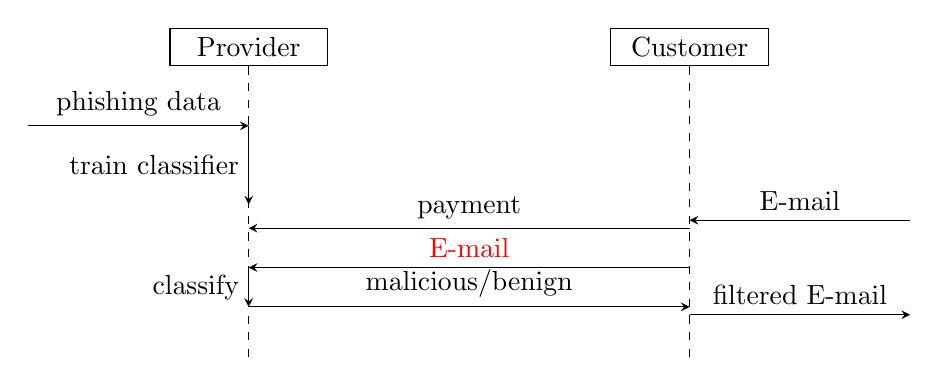
\begin{tikzpicture}[>=stealth,xscale=0.7]
        \draw (-4,0) node[draw, minimum width=2cm] (provider) {Provider};
		\draw[dashed] (provider) -- ++(0,-4);

        \draw (4,0) node[draw, minimum width=2cm] (customer) {Customer};
		\draw[dashed] (customer) -- ++(0,-4);

		\draw[->] (-8,-1) -- (-4,-1) node[above, midway] {phishing data};
		\draw[->] (-4,-1) -- (-4,-2) node[left, midway] {train classifier};

		\draw[->] (8,-2.2) -- (4,-2.2) node[above, midway] {\mail{}};
		\draw[->] (4,-2.3) -- (-4,-2.3) node[above, midway] {payment};
		\draw[->] (4,-2.8) -- (-4,-2.8) node[above, midway] {\textcolor{red}{\mail{}}};
		\draw[->] (-4,-2.8) -- (-4,-3.3) node[left, midway] {classify};
		\draw[->] (-4,-3.3) -- (4,-3.3) node[above, midway] {malicious/benign};
		\draw[->] (4,-3.4) -- (8,-3.4) node[above, midway] {filtered \mail{}};
    \end{tikzpicture}
    \caption{Phishing detection service using an online oracle}
    \label{fig:online-phishing}
\end{figure}


\begin{figure}[h]
    \centering
    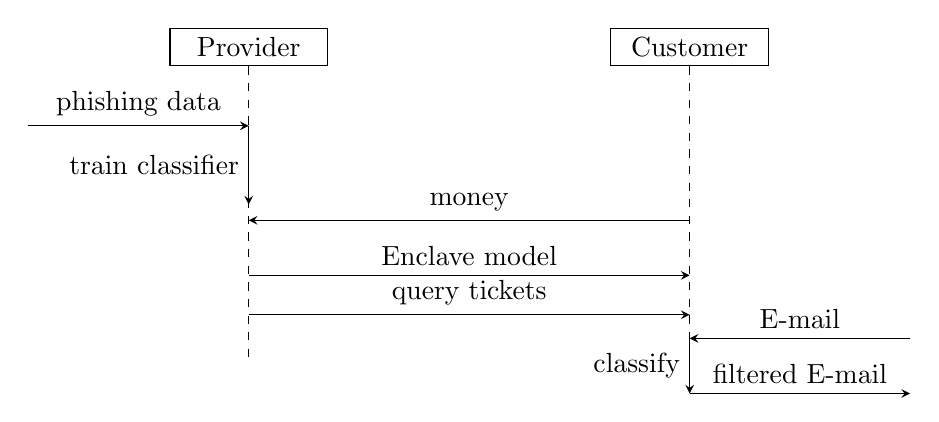
\begin{tikzpicture}[>=stealth, xscale=0.7]
        \draw (-4,0) node[draw, minimum width=2cm] (provider) {Provider};
		\draw[dashed] (provider) -- ++(0,-4);

        \draw (4,0) node[draw, minimum width=2cm] (customer) {Customer};
		\draw[dashed] (customer) -- ++(0,-4);

		\draw[->] (-8,-1) -- (-4,-1) node[above, midway] {phishing data};
		\draw[->] (-4,-1) -- (-4,-2) node[left, midway] {train classifier};

		\draw[->] (4,-2.2) -- (-4,-2.2) node[above, midway] {money};
		\draw[->] (-4,-2.9) -- (4,-2.9) node[above, midway] {Enclave model};
		\draw[->] (-4,-3.4) -- (4,-3.4) node[above, midway] {query tickets};

		\draw[->] (8,-3.7) -- (4,-3.7) node[above, midway] {\mail{}};
		\draw[->] (4,-3.7) -- (4,-4.4) node[left, midway] {classify};
		\draw[->] (4,-4.4) -- (8,-4.4) node[above, midway] {filtered \mail{}};
    \end{tikzpicture}
    \caption{Phishing detection service using an offline oracle inside the enclave}
    \label{fig:offline-phishing}
\end{figure}

\section{Experimental Setup}
\label{sec:setup}

Image recognition tasks as well as text classification tasks are used for testing.
The image recognition tasks are MNIST~\cite{noauthor_mnist_nodate} using a small CNN, and MIT67~\cite{quattoni_recognizing_nodate} using a pretrained VGG16 network as feature extractor.
I fixed the weights for the VGG16 feature extractor during training of the fully connected layers.
For the text classfication we used IMDB review sentiment classification~\cite{maas_learning_2011} using MLPs, and Rotten Tomatoes review sentiment classification~\cite{noauthor_sentiment_nodate} using CNNs on sequences.
The code for these is taken from a Google Text classification tutorial~\cite{noauthor_googleeng-edu_nodate}.
This choice of datasets provides us with CNNs with a reasonably high number of trainable parameters for multiple media types, as well as smaller models for each media type.

For measuring the inference time we cut off the last $n$ layers and converted it to run inside the trusted enclave.
The rest was run in vanilla \tf{}.
We then ran inference on a single input, measuring the time it took for \tf{} to process the input.
This measurement method means we include the setup time for \tf{}, which can be seconds if the inference is done on GPU.
Using the \tf{} output as an input, we measured the time spent on computation inside the enclave, as well as the time it takes to set it up and tear it down.
To separate the impact from running inside the enclave from the impact caused by our implementation and the CPU in general, we also ran the second part of inference in native C.
The difference between native C and the trusted enclave is the extra "penalty" incurred by running the model inside a trusted enclave.

The reported results are averaged over 5 runs.

\section{Experiment Results}
\label{sec:results}

We do have some results

\subsection{TODO: Retraining performance (Not in final paper)}

I did some experiments with fine tuning and freezing.
Unfreezing the weights in the feature extractor during initial training is detrimental to performance, detroying any benefit that would be gained from using a pretrained feature extractor.
However, training the fully connected layers for 500 epochs, unfreezing the weights in the feature extractor, and then training the whole model with a reduced learning rate yields an accuracy increase.
In my tests I fine-tuned the weights using a stochastic gradient descent optimizer for 2000 epochs, once with fixed VGG weights and once while retraining the VGG weights as well.
Starting accuracy for both variants was 53.507\%.
Fine-tuning with VGG weights fixed plateaued at roughly 57.5\%, while fine-tuning all weights reached an accuracy of 64.5\%.

This might be because the feature extractor has been trained on a general purpose dataset and is now being used on a specific scene recognition dataset.
Zhou et al.~\cite{zhou_learning_2014} have studied this problem and provide a different set of weights for the VGG feature extractor specific for scene recognition.
I will try these weights in the future, but they have to be transformed from Caffe to \tf{}.

\section{Discussion}
\label{sec:discussion}

\section{Conclusion}
\label{sec:conclusion}

\bibliographystyle{plain}
\bibliography{Enclave-NN.bib}

\end{document}
